%%%%%%%%%%%%%%%%%%%%%%%%%%%%%%%%%%%%%%%%%%%%%%%%%%%%%%%%%%%%%%%%%%%%%%
% How to use writeLaTeX: 
%
% You edit the source code here on the left, and the preview on the
% right shows you the result within a few seconds.
%
% Bookmark this page and share the URL with your co-authors. They can
% edit at the same time!
%
% You can upload figures, bibliographies, custom classes and
% styles using the files menu.
%
% If you're new to LaTeX, the wikibook is a great place to start:
% http://en.wikibooks.org/wiki/LaTeX
%
%%%%%%%%%%%%%%%%%%%%%%%%%%%%%%%%%%%%%%%%%%%%%%%%%%%%%%%%%%%%%%%%%%%%%%
\documentclass[12pt]{article}
\usepackage{amsmath}

% Set up the images/graphics package
\usepackage{graphicx}
\setkeys{Gin}{width=\linewidth,totalheight=\textheight,keepaspectratio}
\graphicspath{{graphics/}}

% \date{24 January 2009}  % if the \date{} command is left out, the current date will be used
\usepackage{booktabs}
\usepackage{units}
\usepackage{fancyvrb}
\fvset{fontsize=\normalsize}
\usepackage{multicol}
\usepackage{lipsum}
\usepackage{listings}
\usepackage{xcolor}
\usepackage{upquote}
\usepackage{hyperref}

% These commands are used to pretty-print LaTeX commands
\newcommand{\doccmd}[1]{\texttt{\textbackslash#1}}% command name -- adds backslash automatically
\newcommand{\docopt}[1]{\ensuremath{\langle}\textrm{\textit{#1}}\ensuremath{\rangle}}% optional command argument
\newcommand{\docarg}[1]{\textrm{\textit{#1}}}% (required) command argument
\newenvironment{docspec}{\begin{quote}\noindent}{\end{quote}}% command specification environment
\newcommand{\docenv}[1]{\textsf{#1}}% environment name
\newcommand{\docpkg}[1]{\texttt{#1}}% package name
\newcommand{\doccls}[1]{\texttt{#1}}% document class name
\newcommand{\docclsopt}[1]{\texttt{#1}}% document class option name

%New colors defined below
\definecolor{codegreen}{rgb}{0,0.6,0}
\definecolor{codegray}{rgb}{0.5,0.5,0.5}
\definecolor{codepurple}{rgb}{0.58,0,0.82}
\definecolor{backcolour}{rgb}{0.95,0.95,0.92}

%Code listing style named "codestyle"
\lstdefinestyle{codestyle}{
  backgroundcolor=\color{backcolour},
  belowcaptionskip=0.5em,
  belowskip=3em,
  commentstyle=\color{codegreen},
  keywordstyle=\color{magenta},
  numberstyle=\tiny\color{codegray},
  stringstyle=\color{codepurple},
  basicstyle=\fontsize{9}{13}\selectfont\ttfamily,
  breaklines=false,
  breakindent=0pt,
  breakatwhitespace,                 
  columns=fullflexible,
  captionpos=t,                    
  keepspaces=true,                 
  numbers=left,                    
  numbersep=6pt,                  
  showspaces=false,                
  showstringspaces=false,
  showtabs=false,                  
  tabsize=2,
  literate={-}{-}1
}

%"codestyle" code listing set
\lstset{style=codestyle}

\setlength{\oddsidemargin}{0.25in}
\setlength{\textwidth}{6.5in}
\setlength{\topmargin}{0in}
\setlength{\textheight}{8.5in}

%\geometry{showframe}% for debugging purposes -- displays the margins
% \date{24 January 2009}  % if the \date{} command is left out, the current date will be used


\begin{document}

\title{Setting Up a Sustainable Python Research Environment}
\author{Jonathan Thompson (\href{mailto:jthomps8@uccs.edu}{jthomps8@uccs.edu})}

\maketitle% this prints the handout title, author, and date

\begin{abstract}
\noindent This document provides guidance for setting up a sustainable and maintainable local research environment
in Python. It is intended to be accessible to those with little to no familiarity with Python or programming languages
in general while serving as a useful project reference for individuals who regularly utilize Python in their
day-to-day life. Only basic familiarity with computers and their operation is assumed of the reader. Moreover, while
this document does provide background and motivation for the project setup, it is perfectly acceptable to simply run
through the commands as presented in order to get up and running without regard for why the environment works.
Functionality is, after all, the primary motivation for this guide. A sequential list of the commands used in this guide
can be found in Appendix A to this end.

\end{abstract}

%\printclassoptions

The Python programming language is ubiquitous in data science research due to its accessibility as a programming
language, extensive cross-platform support, and open ecosystem of support libraries. In particular, extensive resources
have been invested into optimizing various numerical and scientific computation libraries for Python in no small part
due to the recent explosion of academic and commercial interest in machine learning. For these reasons, a Python
environment serves as an excellent place to begin exploring data science in a concrete setting.\footnote{The reader is
of course encouraged to explore other computational languages in addition to Python (such as MATLAB, Julia, R, etc.) to
determine which may be best for their particular research.} Python's accessibility and ease-of-use does, however, make
it quite easy for one to assemble a Python environment which is a mishmash of the various guides, tutorials, and videos
which are widely available. Each of these guides tends to be flavored by the author's particular background, experience,
and preferences and as such, the resulting environment can quickly become difficult to navigate. While such biases are
bound to be present in any guide, the focus of this document is to create an environment which is simple,
follows industry best-practices, and most importantly may be extended to as many environments as possible.
We begin by installing Python.



\section{Installation}\label{sec:installation}

There is no shortage of "right" ways to install Python, \footnote{There is also no shortage of "wrong" ways, however
- these are the ways which have you scratching your head wondering what on earth you were thinking when you come back
to a dusty project several months later, or which cause the reader to experience great relief upon shutting down their
computer.} and these are of course unique to one's preferred operating system, available computational resources, 
permissions, etc. This guide is designed to be compatible with any pre-existing Python environments which the reader
may already have. To check whether your system already has an existing Python installation (and which Python version is 
installed), run the following in your terminal: \footnote{
    On Windows, this corresponds to the Command Prompt application, which can be accessed via the Start Menu. On
    MacOS/Linux, this corresponds to the Terminal application.
}

\begin{lstlisting}[language=bash, caption=Python Version (Windows)]
C:\Users\MathyMcMathFace> python3 --version
Python 3.10.2
\end{lstlisting}

\begin{lstlisting}[language=bash, caption=Python Version (MacOS/Linux)]
$ python3 --version
Python 3.10.2
\end{lstlisting}

If the above command for your system fails or reports an version of Python which is older than 3.4, you will need to install a 
new Python distribution; we recommend the following sources for their ease-of-use and simplicity:

\subsection{Windows}\label{sec:installation-windows}

We recommend installing Python for Windows through the Windows Store by opening a Command Prompt and 
typing \texttt{python} followed by the \texttt{[Enter]} key, which will automatically take you to
the correct application page in the Windows Store. Alternatively, the following
link will take you directly to the Python application page:
\url{https://www.microsoft.com/store/productId/9PJPW5LDXLZ5}.

Simply click the \texttt{Get} button and wait for installation to complete.

\subsection{MacOS}\label{sec:installation-mac-os}

The latest Python versions for MacOS may be installed by navigating to \url{https://www.python.org/downloads/} in your
favorite browser, clicking the \texttt{Download Python 3.x.x} button (\texttt{3.10.2} at the time of writing) on that 
page, and running the downloaded executable. The installation process is standard fare; accepting the default options 
during the installation process will result in a perfectly fine research environment.

\subsection{Linux}\label{sec:installation-linux}

We recommend that you install Python via your distribution's package manager:\footnote{
    Most modern Linux distributions ship with Python pre-installed; in the event that your system does not have a Python
    distribution, you probably know more about your Linux installation than we do.
}

\begin{lstlisting}[language=bash, caption=Debian/Ubuntu]
$ sudo apt install -y python3
\end{lstlisting}

\begin{lstlisting}[language=bash, caption=Fedora]
$ sudo dnf install -y python3
\end{lstlisting}

\begin{lstlisting}[language=bash, caption=Arch Linux]
$ sudo pacman -S python
\end{lstlisting}

The success of your installation can be verified by opening a new terminal and running the above version command.


\section{Package Management}\label{sec:package-management}

While Python itself is certainly useful out of the box, it does not take long for one to realize that there are a great
many algorithms and functionalities that would be useful in several areas of research. One might think that it would be
quite convenient if there existed a way to write such algorithms once and for all and subsequently share them across
multiple projects. As it turns out, Python provides a mechanism for precisely this by way of a package
management system called \texttt{pip}.\footnote{
    Python is far from unique in this aspect - nearly every programming language in existence today has its own package
    manager(s) for this purpose.
} \texttt{pip} is included in all Python distributions from version \texttt{3.4+}, and as such will serve us quite
conveniently as we explore specialized Python packages which are particularly useful for mathematical computation.
\footnote{
    \texttt{pip} is also the industry-standard package management system for managing package dependencies in 
    most professional Python projects. We will soon see its utility in the context of research.
}

\section{Virtual Environments\label{sec:virtual-environments}}
One advantage to working with a popular open-source software such as Python is that there exists a rich ecosystem
consisting of packages that do much of what one might think of to do with software. Because these packages are typically
maintained by someone else, however, one cannot always be sure that code written against a particular package version
will always run correctly against every subsequent version of the package that is published. Moreover, it may be the
case that two projects are actually incompatible with different versions of the same package, and that installing a
single package version for all projects must necessarily break one or the other.\footnote{
    The ideal solution is naturally to update one or the other projects in order to make them both compatible with the 
    same package version. In practice, however, this tends to involve a cost-benefit analysis that rarely ends in favor 
    of updating the projects.
} Upon consideration, one might come to the conclusion that it would be convenient if there existed some way to isolate
one project's dependencies from another to prevent this sort of thing from happening. A moment's thought will convince 
the reader that it would additionally be convenient if such a mechanism also were to provide a way to explicitly list 
the packages upon which the project depends along with the package versions known to work with the project. Python again 
comes to the rescue with virtual environments.\footnote{
    In contrast to \texttt{pip}, it is unfortunately less common for other languages to provide mechanisms out of the box
    which are analogous to virtual environments.
}
Virtual environments are designed to solve the project dependency management problem, and provide a convenient way to
ensure that projects are reproducable across operating systems and machines.\footnote{
    There is of course sometimes behavior which must necessarily be different across operating systems or hardware, but
    these differences are usually constrained to packages designed to work with particular hardware.
} When operating the context of a virtual environment (which we refer to as \emph{activating} the virtual environment, for 
reasons which will be evident in short order), packages installed with \texttt{pip} will only be installed into
the project directory (folder), and will not affect the environment of any other existing or new Python projects on the
system.

We now proceed to set up a single virtual environment for research. The advantage to a single environment is two-fold:
First, by installing to a single virtual environment, we only have to install any particular package once in order for 
all our projects to be able to use the package. Since it's more common that we wish to use one version across multiple
projects than it is for a project to require its own specific version, we defer the creation of multiple virtual 
environments to those projects which require specific package versions. The second advantage is that if we wish to share
some aspect of our research, we need only share the project files and the file which contains the project's dependencies
and their respective package versions.\footnote{
    By convention, this file is named \texttt{requirements.txt} and resides in the
    project's root folder.
}

We begin by creating a new folder for our research. We use a folder named \texttt{research} in the user
home\footnote{
    The user home directory is where any terminal - Windows or UNIX - will open to by default and hence serves as a
    convenient location for frequently-used files.
} directory, though this choice is of course arbitrary.

\pagebreak
Except where commands differ between Linux and Windows, we will
omit Linux command(s) for the sake of brevity.\footnote{
    A full list of the commands used for each operating system is included in Appendix A.
}


\begin{lstlisting}[language=bash, caption=Create Research Directory (Windows)]
C:\Users\MathyMcMathFace> mkdir research
C:\Users\MathyMcMathFace> cd research
\end{lstlisting}

We now create our virtual environment in a new (also arbitrarily named) \texttt{python-projects} directory:

\begin{lstlisting}[language=bash, caption=Create Virtual Environment (Windows)]
C:\Users\MathyMcMathFace\research> python3 -m venv python-projects/venv
C:\Users\MathyMcMathFace\research> cd python-projects
\end{lstlisting}

The last step is to \emph{activate} our virtual environment. This informs your terminal that it should now look in the
virtual environment for installed packages and commands, and must be done each time you wish to run a command in the
context of your virtual environment.\footnote{
    For instance, if you restart your computer, open a new terminal, etc.
} Only a single virtual environment may be activated at a time
in any given terminal window.

\begin{lstlisting}[language=bash, caption=Activate Virtual Environment (Windows)]
C:\Users\MathyMcMathFace\research\python-projects> .\venv\Scripts\activate
\end{lstlisting}

\begin{lstlisting}[language=bash, caption=Activate Virtual Environment (MacOS/Linux)]
[~/research/python-projects]$ source ./venv/bin/activate
\end{lstlisting}

At this point, we are ready to install any package we may wish via \texttt{pip}. For the sake of clarity, whenever a
command is to be executed within the context of a virtual environment it will be preceded by 
\texttt{(venv)}. It should be understood that such commands execute in a terminal from the 
\texttt{python-projects} directory\footnote{
    Or equivalent, if the virtual environment was installed to a directory other than the one suggested in this guide.
} created in this guide.

\section{Jupyter Notebooks}\label{sec:jupyter-notebooks}

It is at this juncture that we finally utilize the virtual environment we have created for applications specific to 
data science and computational mathematics. We do this by working within the context of a Jupyter Notebook, which
is a web-based development environment which intersperses Python code blocks, Markdown, TeX in order to provide a
cohesive workflow for data science and exploratory computation.

\subsection{Installing Dependencies}\label{sec:jupyter-notebooks-installing-dependencies}

We begin by installing Jupyter itself alongside several useful computational 
packages which are ubiquitous in computational Python:

\begin{lstlisting}[language=bash, caption=Computational Python Libraries (Windows)]
(venv) pip install jupyterlab scipy numpy matplotlib scikit-learn pandas ipywidgets
\end{lstlisting}


\subsection{Saving Dependencies}\label{sec:jupyter-notebooks-saving-dependencies}
To lock our project dependencies and their versions into place, we save them to \texttt{requirements.txt};\footnote{
    To install dependencies from a \texttt{requirements.txt} file in another project or virtual environment, simply run 
    \texttt{pip install -r requirements.txt}.
} This should be done any time \texttt{pip} is used to install or update a package in this virtual environment:

\begin{lstlisting}[language=bash, caption=Save Project Dependencies (Windows)]
(venv) pip freeze > requirements.txt
\end{lstlisting}

\subsection{Starting Jupyter}\label{sec:jupyter-notebooks-starting-jupyter}

The last step is to start the Jupyter server:

\begin{lstlisting}[language=bash, caption=Starting Jupyter (Windows)]
(venv) jupyter notebook
\end{lstlisting}

\pagebreak
Once your Jupyter server has started, navigate to \url{http://localhost:8888/lab} in your browser.
To verify everything is running correctly, create a new notebook:

\begin{figure*}[h]
  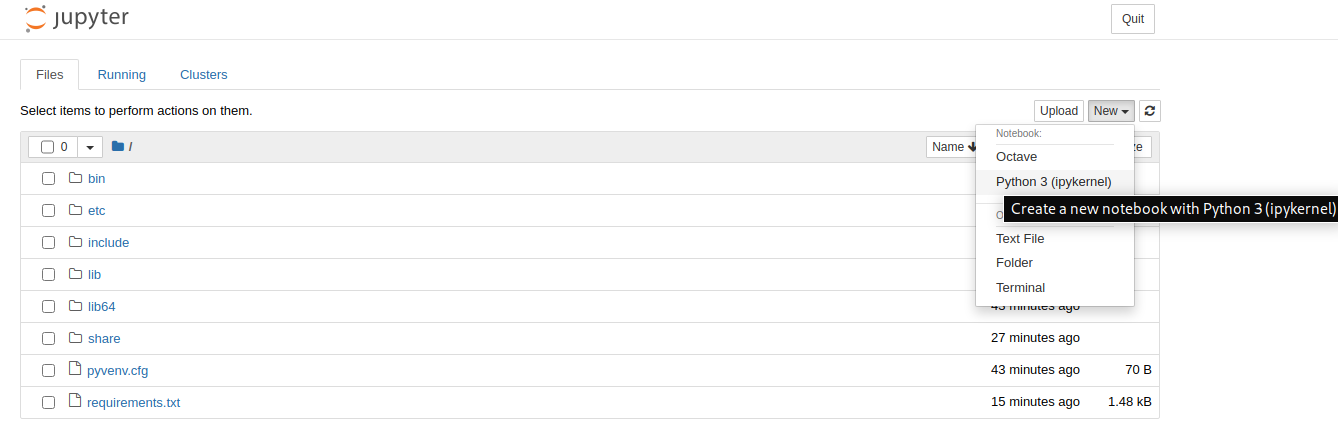
\includegraphics[width=\linewidth]{jupyter_home_new_notebook.png}%
\end{figure*}

In your new notebook, paste the following into the empty code cell and click the \texttt{Run} button:

\begin{lstlisting}[language=Python, caption=Simple Sine Wave]
# Import newly-installed libraries
import matplotlib.pyplot as plt
import numpy as np

# Data for plotting
t = np.arange(0.0, 2.0, 0.01)
s = 1 + np.sin(2 * np.pi * t)

fig, ax = plt.subplots()
ax.plot(t, s)

ax.set(xlabel='time (s)', ylabel='voltage (mV)', title='Simple Sine Wave')
ax.grid()
\end{lstlisting}

You should see the following output:

\begin{figure*}[h]
  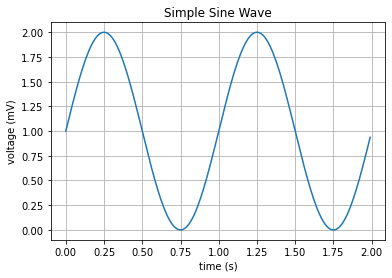
\includegraphics[width=0.34\columnwidth]{jupyter_simple_sine_wave.png}%
\end{figure*}

\pagebreak
\subsection{Returning to Your Virtual Environment}\label{sec:jupyter-notebooks-returning}

Whenever you have exited your virtual environment (e.g., by running the above \texttt{deactivate} command in a virtual
environment, rebooting, or closing all activated terminals), you must re-activate your virtual environment in order to
run Python commands (e.g., \texttt{jupyter notebook}) by navigating to the directory your virtual environment was
 created in (\texttt{python-projects}, in our case), and execute whichever of the following commands pertains to your
operating system:

\begin{lstlisting}[language=bash, caption=Activate Virtual Environment (Windows)]
C:\Users\MathyMcMathFace\research\python-projects> .\venv\Scripts\activate
\end{lstlisting}

\begin{lstlisting}[language=bash, caption=Activate Virtual Environment (MacOS/Linux)]
[~/research/python-projects]$ source ./venv/bin/activate
\end{lstlisting}

You will likely want to start your Jupyter server at this point if it's not already
running elsewhere:

\begin{lstlisting}[language=bash, caption=Starting Jupyter (Windows)]
(venv) jupyter notebook
\end{lstlisting}

\pagebreak
\section{Appendix A - Command Reference}\label{sec:appendix-a}

This section contains a brief listing of the commands used to create and activate
virtual environments.

\subsection{Windows}\label{sec:appendix-a-windows}

To create a new virtual environment:

\begin{lstlisting}[language=bash, caption=Create a Virtual Environment (Windows)]
C:\Users\MathyMcMathFace> mkdir research
C:\Users\MathyMcMathFace> cd research
C:\Users\MathyMcMathFace\research> python3 -m venv python-projects/venv
C:\Users\MathyMcMathFace\research> cd python-projects
\end{lstlisting}

To begin working in the virtual environment created by the above commands, navigate to the 
created virtual environment directory (\texttt{python-projects} in our example) and run:

\begin{lstlisting}[language=bash, caption=Activate a Virtual Environment (Windows)]
C:\Users\MathyMcMathFace\research\python-projects> .\venv\Scripts\activate
\end{lstlisting}

Once your virtual environment has been activated, install Jupyter Notebook along with some other
Python libraries which are useful for scientific computation (this need only be done once per virtual
environment):

\begin{lstlisting}[language=bash, caption=Computational Python Libraries (Windows)]
(venv) pip install jupyterlab scipy numpy matplotlib scikit-learn pandas ipywidgets
\end{lstlisting}

Lastly, to start a Jupyter Notebook server inside an activated virtual environment, simply run:

\begin{lstlisting}[language=bash, caption=Start Jupyter Server (Windows)]
(venv) jupyter notebook
\end{lstlisting}

\pagebreak
\subsection{MacOS/Linux}\label{sec:appendix-a-macos-linux}

To create a new virtual environment:

\begin{lstlisting}[language=bash, caption=Create a Virtual Environment (MacOS/Linux)]
[~]$ mkdir research
[~]$ cd research
[~/research]$ python3 -m venv python-projects/venv
[~/research]$ cd python-projects
\end{lstlisting}

To begin working in the virtual environment created by the above commands, navigate to the 
created virtual environment directory (\texttt{python-projects} in our example) and run:

\begin{lstlisting}[language=bash, caption=Activate a Virtual Environment (MacOS/Linux)]
[~/research/python-projects]$ source ./venv/bin/activate
\end{lstlisting}

Once your virtual environment has been activated, install Jupyter Notebook along with some other
Python libraries which are useful for scientific computation (this need only be done once per virtual
environment):

\begin{lstlisting}[language=bash, caption=Computational Python Libraries (MacOS/Linux)]
(venv) pip install jupyterlab scipy numpy matplotlib scikit-learn pandas ipywidgets
\end{lstlisting}

Lastly, to start a Jupyter Notebook server inside an activated virtual environment, simply run:

\begin{lstlisting}[language=bash, caption=Start Jupyter Server (MacOS/Linux)]
(venv) jupyter notebook
\end{lstlisting}

\end{document}